
\section{Standard Model Particles}
\label{sec:relatedWorks:smParticles}

% What is the world made of? Throughout the history, numerous theories were developed to answer the question. The ancient Greeks modeled the matter with four fundamental elements: air, water, fire, and earth, while the ancient Chinese believed in the five most essential building blocks: metal, wood, water, fire, and earth. In the modern age, the emergence of science provides a systematic approach to develop and test these models. As the experimental technology allows us to probe smaller and smaller structures, our understanding of the fundamental elements of matter evolves from molecules to atoms, then to nucleons and electrons, finally to quarks and leptons. This level of understanding was achieved by a set of exciting progress in both physics theory and experiments in the most recent century, which together led us to the Standard Model (SM), a systematic and elegant answer to the question of "what is matter", as well as "what is force".

% Standard Model (SM), since its establishment, has been very successful in making predictions for the experiments, such as the existence, properties, and behaviors of particles. On the other hand, it has been tested with remarkably high precision in many aspects in experiments such as fixed-target experiments, collider experiments, and neutrino experiments. Despite its tremendous success, SM is still not the perfect ultimate theory to settle down because it still has many limitations: the gravitational force which is one of the four fundamental interactions in nature is not included in the SM; the dark matter hinted by many astronomy observations is not modeled by any SM fermions; electromagnetic and weak forces are unified, but it does not unify the strong force; moreover, the running couplings of the three forces do not join at one point in the high energy scale. So seeking new physics beyond the standard model is one of the important topics in particle physics nowadays. 


\begin{figure}[ht]
    \centering
    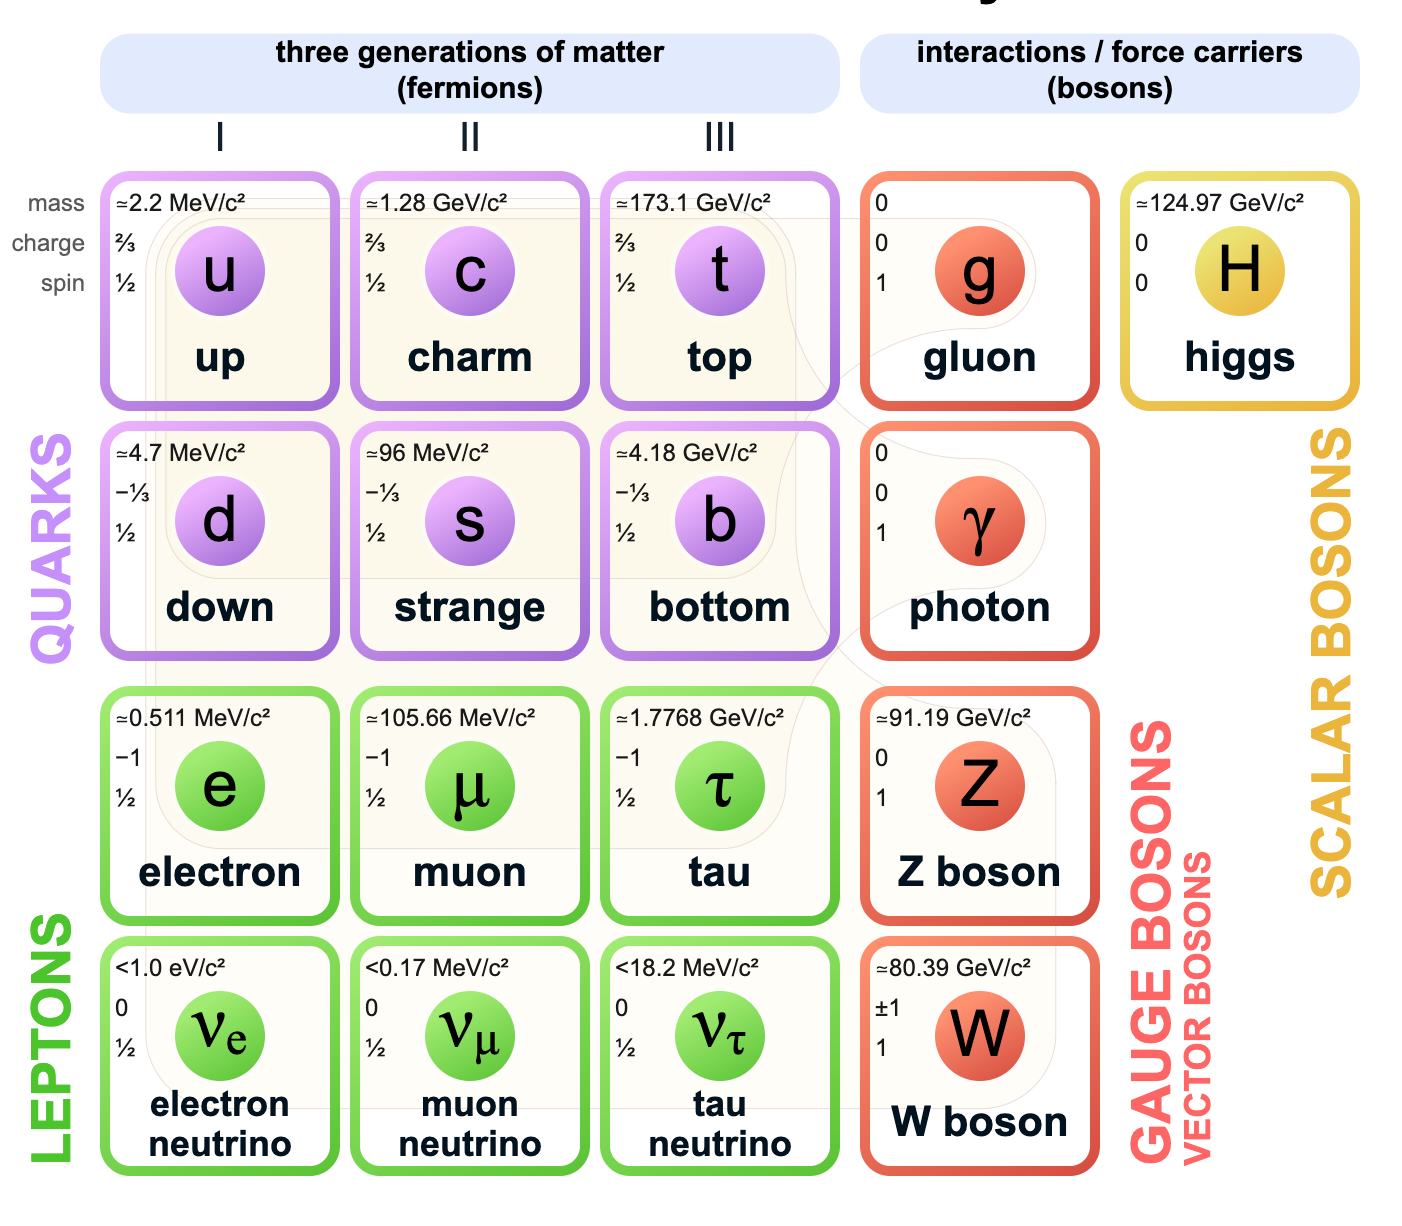
\includegraphics[width=0.6\textwidth]{chapters/RelatedWorks/sectionSMParticles/figures/sm.png}
    \caption{Particles in the Standard Model. Fermions include quarks and leptons both having three generations, while bosons include four gauge bosons and one Higgs boson.}
    \label{fig:relatedWorks:smParticles:sm}
\end{figure}

Standard Model treats matter and the force among the matter as a set of different quantum fields, excited states of which correspond to different fundamental particles. Figure~\ref{fig:relatedWorks:smParticles:sm} shows the table of SM particles. The ``matter particles" are  spin-$\frac{1}{2}$ fermions including quarks and leptons, both having three generations. The ``force particles" are spin-1 gauge bosons accounting for the electromagnetic, strong, weak forces. Additionally, there is a spin-0 Higgs boson that generates mass for fermions and gauge bosons. The theoretical foundation of the SM particles in Figure~\ref{fig:relatedWorks:smParticles:sm} is the quantum field theory (QFT), a theory joining quantum mechanics and special relativity.  A QFT description for the SM is included in Section~\ref{sec:relatedWorks:qft}, covering Yang-Mills Gauge Theory, Higgs Mechanism, Glashow-Weinberg-Salam (GWS) electroweak model and Quantum Chromodynamics (QCD). This section provides an overall description of the SM particles. 


\subsection{Fermions}
\label{sec:relatedWorks:smParticles:fermion}

\begin{table}[ht]
    \centering
    \setlength{\tabcolsep}{1 em}
    \renewcommand{\arraystretch}{1.5}
    \caption{The electroweak quantum number of the first generation of the leptons and quarks. The second and third generation have the same EW quantum number as the first generation. The quantum numbers are isospin $T$, the third component of isospin $T^3$, charge $Q$ and hypercharge $Y$. }
    \resizebox{\textwidth}{!}{
    \begin{tabular}{ccccc|ccccc}
    \hline
    lepton      & $T$           & $T^3$          & $Q$ & $Y$ & quark  & $T$           & $T^3$          & $Q$            & $Y$            \\
    \hline
    $\nu_{e,L}$ & $\frac{1}{2}$ & $\frac{1}{2}$  & 0   & -1  & $u_L$  & $\frac{1}{2}$ & $\frac{1}{2}$  & $\frac{2}{3}$  & $\frac{1}{3}$  \\
    $e_L$       & $\frac{1}{2}$ & $-\frac{1}{2}$ & -1  & -1  & $d_L$  & $\frac{1}{2}$ & $-\frac{1}{2}$ & $-\frac{1}{3}$ & $\frac{1}{3}$  \\
    \hline
    -           & -             & -              & -   & -   & $u_R$  & 0             & 0              & $\frac{2}{3}$  & $\frac{4}{3}$  \\
    $e_R$       & 0             & 0              & -1  & -2  & $d_R$  & 0             & 0              & $-\frac{1}{3}$ & $-\frac{2}{3}$ \\
    \hline
    \end{tabular}}
    \label{tab:relatedWorks:smParticles:ewQuantumNumber}
\end{table}


\textbf{Quarks}. Three generations of quarks have been discovered: up ($u$) and down ($d$) being the first generation, charm ($c$) and strange ($s$) being the second generation, top ($t$) and bottom ($b$) being the third generation. The terminology ``generation" is often referred to as ``family" as well. The up, charm and top quarks have electric charge of $-\frac{2}{3}$, while the electric charge of down, strange, and bottom quark is $\frac{1}{3}$. Other than electric charge, a quark also carries color quantum number and thus participates in the strong interaction. The color quantum number in the strong force including red, green, and blue, is analogous to the electric charge in the electromagnetic force. Each quark has its corresponding antiquark carrying an opposite electric charge and anti-color. However, neither the fractional charge nor individual color charge is observed in nature, because quarks never exist alone. Quarks and their properties only reveal during the high-energy short-distance local interactions. In the low energy scale, they are always combined in two-quark or three-quark bounded states, called mesons and baryons respectively, which are color-neutral and integer-charged. This phenomenon is the so-called quark confinement, the mathematical form of which is presented in Section~\ref{sec:relatedWorks:qft:qcd}. Quarks not only couple to the electromagnetic and strong force, but are also involved in the weak interaction. The weak hypercharge and isospin of quarks are listed in the Table~\ref{tab:relatedWorks:smParticles:ewQuantumNumber}. The masses of quarks arrange from a few MeV to 173 GeV, increasing with the quark generations. The heavy quarks have a short lifetime and decay into light quarks via the weak force with quark mixing. Therefore, the matter in our everyday life includes only the first generation light quarks. The most massive quark $t$ decays almost instantaneously to a $b$ quark and a weak gauge boson upon its production before hadronizing into bounded states. Quark model has been successful in the classification of mesons and baryons, and explaining the observations in many experiments such as the lepton-nucleon deep-inelastic scattering, electron-positron annihilation and proton-proton hard collision.



\textbf{Leptons}. Three generations leptons have been discovered: electrons ($e$) and electron neutrino ($\nu_e$) being the first generation, muon ($\mu$) and muon neutrino ($\nu_\mu$) being the second generation, tau ($\tau$) and tau neutrino ($\nu_\tau$) being the third generation. Electron, muon, and tau have -1 electric charge and thus couple to the electromagnetic force, while all neutrinos are not charged and do not interact electromagnetically. Charged leptons can be both left-handed and right-handed, while the neutrinos can only be left-handed because right-handed neutrinos have not been experimentally observed so far. Due to the chiral nature of weak interaction, the left-handed leptons couples to both W and Z weak gauge bosons, while right-handed charged leptons have zero weak isospin and do not couple to the W boson. The quantum number of leptons are also shown in the Table~\ref{tab:relatedWorks:smParticles:ewQuantumNumber}. The masses of the charged leptons increases with the lepton generations. Charged leptons in the second and third generations have finite lifetimes. Therefore, electrons are the only charged lepton in our everyday matter. The mass of neutrinos in the Standard Model had been thought of as zero until the discovery of neutrino oscillation. The neutrino masses were then added to the SM. But the exact values of neutrino masses are still not fully determined yet. 




\subsection{Boson}
\label{sec:relatedWorks:smParticles:boson}

The bosons in the SM consist of four spin-1 gauge bosons and one spin-0 Higgs boson. Four gauge bosons are responsible for the forces between fermions: the electromagnetic force is mediated by the photon $\gamma$; the strong nuclear force is propagated by gluons $g$, the weak force is carried by the $W^\pm$ and $Z$ bosons. In the QFT, the existence of gauge boson originates from engaging the local symmetries or gauge symmetry to the fermions Lagrangian. In other words, force is modelled as the consequence of gauging the matter. The gauge symmetry is further discussed in Section~\ref{sec:relatedWorks:qft:gaugeSymmetry}. Among the four gauge bosons, photon and gluon are massless while the $W\pm$ and $Z$ boson are massive with $m_W = 80.385\pm0.015$ GeV and $m_Z = 90.183\pm 0.002$ GeV \cite{pdg2020} respectively. The non-zero mass of the gauge boson breaks the gauge symmetry and causes renormalization issue, unless the mass of gauge boson is generated by the Higgs mechanism, discussed in Section~\ref{sec:relatedWorks:qft:higgsMechanism}. The Higgs boson is a spin-0 boson predicted in the 1960s to solve the issues related to the gauge boson mass. It was finally confirmed exist at $m_H=125.09\pm 0.24$ \GeV by the CMS \cite{Chatrchyan:2012ufa} and the ATLAS \cite{Aad:2012tfa} experiment at LHC in 2012. It was the last missing piece added in the SM particles, which completes the table in Figure~\ref{fig:relatedWorks:smParticles:sm}. Besides the mass of gauge bosons, the Higgs boson also generates the mass for all the fermions via Yukawa couplings.

